\PassOptionsToPackage{svgnames}{xcolor}
\documentclass[a4paper]{article}
\usepackage[margin=2.5cm]{geometry}
%\documentclass[journal]{IEEEtran}
%\documentclass{report}
%\documentclass{ActaOulu}

\usepackage{fontenc}[T1]
\usepackage{alltt}
%\usepackage{epsfig}
\usepackage{graphicx}

\usepackage[english]{babel}
\usepackage{url}
\usepackage{multirow}
\graphicspath{{figures/}}
\usepackage{subfig}
\usepackage{hyperref}
\usepackage{amsthm}
	\newtheorem{mydef}{Definition}

\usepackage{verbatim}
\usepackage{multirow}
\usepackage{booktabs}
\usepackage{amsmath}
\usepackage{amsfonts}
\usepackage{amssymb}
\usepackage{hyperref}
\usepackage{breakurl}
\usepackage{mdwlist}
\usepackage[ruled,vlined,linesnumbered]{algorithm2e}
% \usepackage{color}
\usepackage{pgf}
\usepackage{tikz}
\usetikzlibrary{shapes,arrows,shapes.multipart,positioning, fit, calc}
\usepackage{longtable}
\usepackage{enumitem}

%For code listings:
\usepackage{listings}
\usepackage{lstcustom}
\usepackage[scaled=0.8]{beramono}% beramono or luximono give very nice ttfamily fonts
% \usepackage{lmodern}
\usepackage{courier}



%For color boxes:
\usepackage{tcolorbox}
\tcbuselibrary{skins,breakable}
\usetikzlibrary{shadings,shadows}

\usepackage{xcolor}
\definecolor{lightBlueCodeBlock}{HTML}{EBEBF8}
\definecolor{darkBlueCodeBlock}{HTML}{D7D7F0}
\definecolor{blueTitleCodeBlock}{HTML}{4545b9}
\definecolor{purpleNodeColor}{HTML}{BA55D3}


\newenvironment{myexampleblock}[1]{%
    \tcolorbox[beamer,%
    noparskip,breakable,
    colback=LightGreen,colframe=DarkGreen,%
    colbacklower=LimeGreen!75!LightGreen,%
    title=#1]}%
    {\endtcolorbox}

\newenvironment{myalertblock}[1]{%
    \tcolorbox[beamer,%
    noparskip,breakable,
    colback=LightCoral,colframe=DarkRed,%
    colbacklower=Tomato!75!LightCoral,%
    title=#1]}%
    {\endtcolorbox}

\newenvironment{myblock}[1]{%
    \tcolorbox[beamer,%
    noparskip,breakable,
    colback=lightBlueCodeBlock,colframe=darkBlueCodeBlock,%
    colbacklower=darkBlueCodeBlock!75!lightBlueCodeBlock,%
    coltitle=blueTitleCodeBlock,
    title=#1]}%
    {\endtcolorbox}


\newcommand{\code}[1]{\lstinline[language=java, style=seminar]!#1!}


\tikzset{
  treenode/.style = {align=center, inner sep=0pt, text centered,
    font=\sffamily},
  blackNode/.style = {treenode, circle, black, font=\sffamily\bfseries, draw=black, text width=1.5em},% arbre rouge noir, noeud noir
  greenNode/.style = {treenode, circle, green, draw=green, text width=1.5em, very thick},% arbre rouge noir, noeud rouge
  purpleNode/.style = {treenode, circle, purpleNodeColor, draw=purpleNodeColor, text width=1.5em, very thick},% arbre rouge noir, noeud rouge
}


\begin{document}

\title{Branch-and-Price Framework in jORLib}
\author{Joris Kinable}
\date{\today}

\maketitle
\section{Introduction}
When reading about Column Generation or Branch-and-Price in math books, the procedures are always very clear: define a Master and a Pricing Problem, and solve them iteratively until optimality is reached. If the solution is fractional: branch. The reality is however significantly more complex. The quality of any Column Generation procedure significantly depends on the many implementation choices one has to make. These design choices, as well a many other important details are frequently omitted when discussing Column Generation:
\begin{enumerate}
 \item how to obtain an initial subset of columns?
 \item in which order should the nodes in the Branch-and-Price tree be processed?
 \item when should we check for violated inequalities in the Master Problem?
 \item should we return one or more columns in the Pricing Problem?
\end{enumerate}
Very often, there does not exist a clear-cut answer to these questions. The only way to find out, is simply by trial-and-error. Implementing a Branch-and-Price approach is a relatively complex and very time consuming task. Designing the approach on paper, implementing a basic implementation, testing and debugging the implementation takes up a considerable portion of the available development time, leaving little time to experiment with different settings or alternative implementation choices. A good framework could significantly reduce the required development time, and in addition, reduce the amount of debugging required.\\
The Column Generation framework in jORLib provides a flexible way to implement Column Generation and Branch-and-Price procedures. The framework does \emph{not} provide any automated means to solve a problem through CG; it merely provides a template for your implementation. To implement a simple CG procedure through this framework, the user is required to provide a definition of the Master Problem, one or more Pricing Problems and corresponding algorithms to solve these Pricing Problems, and, of course, a definition of a Column. More advanced implementations may use features such as: the separation of valid inequalities for the Master Problem, or Branch-and-Price.\\
You do not need to be concerned about structural issues: the framework connects the Master Problem and Pricing Problems, it will solve the Pricing Problems in parallel for you, it provides means to calculate bounds on the Master Problem, Pricing Problem, etc. The Branch-and-Price extension takes care of the Branch-and-Price tree which is implemented as a fully reversible data structure. Consequently, nodes in the Branch-and-Price tree can be processed in arbitrary order. Nodes are pruned when bounds are exceeded.\\ 
The Column Generation and Branch-and-Price framework is designed in such a way that it offers you as much flexibility as possible (nearly every method can be overridden by a custom implementation), while still limiting the amount of code you would have to write to get a working solution. The framework does \emph{not} impose restrictions on the the kind of solver used to solve the Master or Pricing Problems: the master problem may be solved through some Linear Programming solver such as CPLEX, or Gurobi, Ipopt, etc, while the Pricing Problems may be solved in any conceivable way.\\
The remainder of this manual discusses the functionality and structure of the framework, starting off with a number of examples.

\section{Example 1 - Solving the Cutting Stock Problem through Column Generation}\label{sec:cutting_stock}
%This section walks over a number of example implementations to show various aspects of the Branch-and-Price framework.
In the Cutting Stock Problem (CSP), a predefined number of so-called finals of a given size need to be produced. Finals can be cut from raws of fixed size. The goal is to cut all the finals, using the smallest number of raws. For a full description of the problem, including an example, refer to: \url{http://en.wikipedia.org/wiki/Cutting_stock_problem}. Here we will only state the Master Problem and Pricing Problem.\\
Techniques used in this example:
\begin{itemize}
 \item Column generation
\end{itemize}
A full implementation can be found in the demo package.

\subsection{Problem description}
\begin{table}[h]
\begin{tabular}{ll}
\toprule
\textbf{Parameter} 	& \textbf{Description}\\
\midrule
$I$		& Set of cutting patterns. Each cutting pattern describes how to cut a single raw.\\
$J$		& Set of finals\\
$a_{ij}$		& Number of times that final $j\in J$ appears in cutting pattern $i\in I$\\
$d_j$		& Demand for final $j\in J$\\
$w_j$		& Width of final $j\in J$\\
$L$		& Width of a raw\\
\bottomrule
\end{tabular}
\caption{}
\label{tbl:cutting_stock} 
\end{table}

The Master Problem (MP) for Cutting stock is defined as:
\begin{align}
\label{eq:MP_CS.0} \mathit{MP:}\; min\; &\sum_{i\in I} z_i &\\
\label{eq:MP_CS.1} \mbox{s.t. }&\sum_{i \in I} a_{ij}z_i\geq q_j & \forall j\in J\\
\label{eq:MP_CS.2} &z_i\geq 0 &\forall i=1,\dots,n
\end{align}
Here, variable $z_i$ indicates how often pattern $i$ is used. The objective function \eqref{eq:MP_CS.0} states that we want to use as little raws as possible. Constraints \eqref{eq:MP_CS.1} state that sufficient finals of each width $j\in J$ are produced. The dual of the Master Problem (DMP) can be stated as:
\begin{align}
\label{eq:DMP_CS.0} \mathit{DMP:}\; max\; &\sum_{j\in J} q_ju_j &\\
\label{eq:DMP_CS.1} \mbox{s.t. }&\sum_{j\in J} a_{ij}u_j\leq 1 & \forall i\in I\\
\label{eq:DMP_CS.2} &u_j\geq 0 &\forall j\in J
\end{align}
Consequently, the Pricing Problem can be defined as: does there exists a pattern $i\in I$ such that $\sum_{j\in J}a_{ij}u_j>1$? The Pricing Problem can be solved through the following knapsack problem:
\begin{align}
\label{eq:PRICE_CS.0} \mathit{PRICING:}\; max\; &\sum_{j\in J} a_ju_j &\\
\label{eq:PRICE_CS.1} \mbox{s.t. }&\sum_{j\in J} w_ja_j\leq L & \\
\label{eq:PRICE_CS.2} &a_j\mbox{ integer} &\forall j\in J
\end{align}

\subsection{Implementation}\label{subsec:cutting_stock_impl}
The following classes need to be extended to implement Column Generation for the Cutting Stock problem:
\begin{enumerate}[nolistsep]
 \item \code{AbstractColumn} - This class defines a column in the Column Generation process.
 \item \code{AbstractMaster} - This problem defines the Master Problem.
 \item \code{AbstractMasterData} - This class stores data from the Master Problem.
 \item \code{AbstractPricingProblem} - This class defines a Pricing Problem and provides storages for shared data between the Master Problem and the Pricing Problem solvers.
 \item \code{AbstractPricingProblemSolver} - A solver class for the Pricing Problem.
\end{enumerate}
In addition, we need to define a data model class which defines the Cutting Stock problem. \\

In the remainder of this section we discuss each of these classes individually. A complete, working, implementation is provided in the demo package. The actual implementation may deviate from the examples shown below as many of the irrelevant details have been omitted.\\
Lets first start by defining a small class defining our problem. This class will be referred to as \code{dataModel} and will be accessible from all classes in the framework.
\begin{myblock}{CuttingStock}
\begin{lstlisting}[language=java, style=eclipseArticle, xleftmargin=2em]  
public final class CuttingStock implements ModelInterface{
	public final int nrFinals=4; //Number of different finals
	public final int rollWidth=100; //Width of the raws
	public final int[] finals={45, 36, 31, 14}; //Size of the finals
	public final int[] demandForFinals={97, 610, 395, 211}; //Requested quantity of each final

	@Override
	public String getName() { return "CuttingStockExample";}
}
\end{lstlisting}
\end{myblock}
Next up, lets define a column in our Cutting Stock problem. Each column (\code{CuttingPattern}) maintains how many finals of a given width are produced. We will store this information in a '\code{yieldVector}':
\begin{myblock}{CuttingPattern}
\begin{lstlisting}[language=java, style=eclipseArticle, xleftmargin=2em]  
public final class CuttingPattern extends AbstractColumn<CuttingStock, PricingProblem> {
	/** Denotes the number of times each final is cut out of the raw. (vector a_j)**/
	public final int[] yieldVector;

	public CuttingPattern(PricingProblem pricingProblem, boolean isArtificial, String creator, int[] pattern) {
		super(pricingProblem, isArtificial, creator);
		this.yieldVector=pattern;
	}

	@Override
	public boolean equals(Object o) {<Code Omitted>}

	@Override
	public int hashCode() {<Code Omitted>}

	@Override
	public String toString() {<Code Omitted>}
}
\end{lstlisting}
\end{myblock}
The constructor of AbstractColumn takes 3 arguments:
\begin{enumerate}[nolistsep]
 \item \code{String creator}: textual description denoting who created the column, i.e. some algorithm, initial solution etc. This is for debugging purposes to track the origin of the column.
 \item \code{boolean isArtificial} artificial columns may be added to create an initial feasible solution to the Master Problem. artificial columns can never constitute a real solution. 
 \item \code{PricingProblem pricingProblem}: the Pricing Problem to which this column belongs. 
\end{enumerate}
Finally, make sure you implement the \code{equals} and \code{hashCode} methods; failing to implement these correctly may result in undefined behavior.

After defining what a Column is in our problem, we have to define a Master Problem and a Pricing Problem. The Master Problem consists of 7 important parts:
\begin{itemize}[nolistsep]
 \item Constructor - The constructor receives our data model which defines the problem, as well as a reference to our Pricing Problem.
 \item \code{buildModel} method - This method builds the Master Problem, which is usually a linear program defined in CPLEX or Gurobi
 \item \code{solveMasterProblem} method - This method solves the Master Problem
 \item \code{addColumn} method - This method is invoked when a Pricing Problem generates a new column; the column has to be added to the Master Problem
 \item \code{initializePricingProblem} method - This method is invoked after the Master Problem has been solved; The dual information required to solve the Pricing Problem has to be passed to the \code{PricingProblem} object.
 \item \code{getSolution} method - This method returns a list of columns constituting the solution, in our case a list of columns with non-zero $z_i$ values.
 \item \code{close} method - This method is invoked at the end of the Column Generation procedure to close the Master Problem (analogous to destructor in C++).
\end{itemize}
For demonstration purposes, we will assume that the Master Problem is being solved by IBM Cplex, but we would like to emphasize that any kind of solver (Gurobi, Ipopt, CP Optimizer, .... ) may be used.

\begin{myblock}{Master}
\begin{lstlisting}[language=java, style=eclipseArticle, xleftmargin=2em]  
public final class Master extends AbstractMaster<CuttingStock, CuttingPattern, PricingProblem, CuttingStockMasterData> {
	public Master(CuttingStock dataModel, PricingProblem pricingProblem) {
		super(dataModel, pricingProblem, OptimizationSense.MINIMIZE);
	}

	@Override
	protected CuttingStockMasterData buildModel() {
		//Define a container for the variables		
		Map<PricingProblem, OrderedBiMap<CuttingPattern, IloNumVar>> variableMap=...;
		
		//Define objective
		obj= cplex.addMinimize();

		//Define constraint: \sum_{i \in I} a_{ij}z_i>= q_j for all j\in J
		satisfyDemandConstr=new IloRange[dataModel.nrFinals];
		for(int j=0; j< dataModel.nrFinals; j++)
			satisfyDemandConstr[j]= cplex.addRange(dataModel.demandForFinals[j], Integer.MAXVALUE);
		
		//Return a new data object which will hold data from the Master Problem
		return new CuttingStockMasterData(variableMap);
	}

	@Override
	protected boolean solveMasterProblem(long timeLimit) throws TimeLimitExceededException {
		//Set time limit
		double timeRemaining=timeLimit-System.currentTimeMillis())/1000.0;
		cplex.setParam(IloCplex.DoubleParam.TiLim, timeRemaining);
			
		//Solve the model
		if(!cplex.solve() || cplex.getStatus()!=IloCplex.Status.Optimal){
			if(cplex.getCplexStatus()==IloCplex.CplexStatus.AbortTimeLim)
				throw new TimeLimitExceededException();
			else
				throw new RuntimeException("Master Problem solve failed!");
		}else{
			masterData.objectiveValue= cplex.getObjValue();
		}
		return true;
	}

	/**
	 * Store the dual information required by the Pricing Problems into the Pricing Problem object
	 */
	@Override
	public void initializePricingProblem(PricingProblem pricingProblem){
		double[] duals= cplex.getDuals(satisfyDemandConstr);
		pricingProblem.initPricingProblem(duals);
	}

	/**
	 * Function which adds a new column to the Master Problem
	 */
	@Override
	public void addColumn(CuttingPattern column) {
		//Register column with objective
		IloColumn iloColumn= cplex.column(obj,1);
		
		//Register column with demand constraint
		for(int i=0; i< dataModel.nrFinals; i++)
			iloColumn=iloColumn.and(cplex.column(satisfyDemandConstr[i], column.yieldVector[i]));
			
		//Create the variable and store it
		IloNumVar var= cplex.numVar(iloColumn, 0, Double.MAX_VALUE, "z_"+","+masterData.getNrColumns());
		cplex.add(var);
		masterData.addColumn(column, var);
	}

	/**
	 * Return the solution, i.e columns with non-zero z_i values
	 */
	@Override
	public List<CuttingPattern> getSolution() {
		List<CuttingPattern> solution=new ArrayList<>();
		for(CuttingPattern cp : masterData.getColumns()){
			cuttingPatterns[i].value=cplex.getValue(cp);
			if(cuttingPatterns[i].value>=config.PRECISION){
				solution.add(cuttingPatterns[i]);
			}
		}
		return solution;
	}

	@Override
	public void close() {<Code Omitted>}	
}
\end{lstlisting}
\end{myblock}
Data originating from the Master Problem, such as its variables, constraint etc may be required by other classes. A shared object which extends \code{AbstractMasterData} is created for this purpose in the \code{buildModel} method of the Master Problem. This object is for example passed to a \code{CutHandler} to separate violated inequalities (cuts). For our CuttingStock problem, we only store the variables in this object:

\begin{myblock}{CuttingStockMasterData}
\begin{lstlisting}[language=java, style=eclipseArticle, xleftmargin=2em]  
public final class CuttingStockMasterData extends MasterData<CuttingStock, CuttingPattern, PricingProblem, IloNumVar>{
    public CuttingStockMasterData(Map<PricingProblem, OrderedBiMap<CuttingPattern, IloNumVar>> varMap) {
        super(varMap);
    }
}
\end{lstlisting}
\end{myblock}

Next up is the Pricing Problem. For Cutting Stock, there is only one Pricing Problem.  The \code{AbstractPricingProblem} class mainly serves as a container to hold the dual information coming from the Master Problem. It \emph{defines} a Pricing Problem which can be solved by some algorithm. In our case, the \code{PricingProblem} class maintains the $u_j$, $j\in J$ dual values.
\begin{myblock}{PricingProblem}
\begin{lstlisting}[language=java, style=eclipseArticle, xleftmargin=2em]  
public final class PricingProblem extends AbstractPricingProblem<CuttingStock> {
	public PricingProblem(CuttingStock modelData, String name) {
		super(modelData, name);
	}
}
\end{lstlisting}
\end{myblock}
After defining the data object which stores the information required to solve the Pricing Problem, one or more solvers for the Pricing Problem have to be defined. The Pricing Problem of the Cutting Stock problem is a knapsack problem. Each time the Pricing Problem is solved, only the objective changes ($max\; \sum_{j\in J} a_ju_j$); the constraint remain the same.

\begin{myblock}{ExactPricingProblemSolver}
\begin{lstlisting}[language=java, style=eclipseArticle, xleftmargin=2em]  
public final class ExactPricingProblemSolver extends AbstractPricingProblemSolver<CuttingStock, CuttingPattern, PricingProblem> {
	public ExactPricingProblemSolver(CuttingStock dataModel, PricingProblem pricingProblem) {
		super(dataModel, pricingProblem);
		this.name="ExactSolver"; //Set a name for the solver
		knapsackSolver=new KnapsackSolver();
	}
	
	@Override
	protected List<CuttingPattern> generateNewColumns() throws TimeLimitExceededException {
		List<CuttingPattern> newPatterns=new ArrayList<>();
		knapsackSolver.solve();
		if(knapsackSolver.getObjective() >= 1+config.PRECISION){ //Generate new column
			int[] pattern=knapsackSolver.getItemCoefficients();
			CuttingPattern column=new CuttingPattern("exactPricing", false, pattern, pricingProblem);
			newPatterns.add(column);
		}
		return newPatterns;
	}

	/**
	 * Set the objective value
	 */
	@Override
	protected void setObjective() {
		//Update the objective function with the new dual values, by using the fields in the pricingProblem, e.g. pricingProblem.dualCosts
		knapsackSolver.setObjective(pricingProblem.dualCosts);
	}

	@Override
	public void close() {<Code Omitted>}
}
\end{lstlisting}
\end{myblock}
Each time the Pricing Problem is solved, the \code{setObjective} function gets invoked first. During the execution of this function, the solver can prepare its data structures and get the new dual information. Next the \code{generateNewColumns} method is invoked which produces zero or more columns. Finally, when the Column Generation procedure terminates, the close() function is invoked which allows for cleanup. It serves the same purpose as a destructor in C++.\\
Finally, we need to bring everything together in a main class.
\begin{myblock}{CuttingStockSolver}
\begin{lstlisting}[language=java, style=eclipseArticle, xleftmargin=2em]  
public final class CuttingStockSolver {
	public CuttingStockSolver(CuttingStock dataModel){

		//Create the Pricing Problem
		PricingProblem pricingProblem=new PricingProblem(dataModel, "cuttingStockPricing");

		//Create the Master Problem
		Master master=new Master(dataModel, pricingProblem);

		//Define which solvers to use
		List<Class<? extends AbstractPricingProblemSolver<CuttingStock, CuttingPattern, PricingProblem>>> solvers= Collections.singletonList(ExactPricingProblemSolver.class);

		//Define an upper bound (stronger is better). In this case we simply sum the demands, i.e. cut each final from its own raw (Rather poor initial solution).
		int upperBound=IntStream.of(dataModel.demandForFinals).sum();

		//Create a set of initial Columns.
		List<CuttingPattern> initSolution=this.getInitialSolution(pricingProblem);

		//Create a column generation instance
		ColGen<CuttingStock, CuttingPattern, PricingProblem> cg=new ColGen<>(dataModel, master, pricingProblem, solvers, initSolution, upperBound);

		//OPTIONAL: add a debugger
		SimpleDebugger debugger=new SimpleDebugger(cg);

		//OPTIONAL: add a logger
		SimpleCGLogger logger=new SimpleCGLogger(cg, new File("./cuttingStock.log"));

		//Solve the problem through column generation
		cg.solve(System.currentTimeMillis()+1000L);

		//Print solution:
		<Code Omitted>
		
		//Clean up:
		cg.close(); //This closes both the master and Pricing Problems
	}
	
	/**
	 * Create an initial solution for the Cutting Stock Problem.
	 */
	private List<CuttingPattern> getInitialSolution(PricingProblem pricingProblem){<Code Omitted>}
}
\end{lstlisting}
\end{myblock}
In the code snippet above, the only new class we have not introduced before is the \code{ColGen} class. This class manages the entire solve procedure by invoking the master and Pricing Problems iteratively. This class is provided as part of the framework; its basic implementation suffices for most use cases. Nevertheless, when desired each of its methods may be overridden by a custom implementation.




\section{Example 2 - Solving the Traveling Salesman Problem through Branch-and-Price}\label{sec:tsp}
In this example, we will solve the well-known Traveling Salesman Problem (TSP) through Branch-and-Price. In the TSP problem, we are looking for a least cost Hamiltonian cycle in a graph. In this particular example we will assume that the number of vertices in the graph is even, and that the graph is undirected.\\
A matching in a graph is defined as a set of edges such that no two edges in the set have an endpoint in common. A matching in a graph is said to be \emph{perfect} if every vertex in the graph is incident to exactly one edge in the matching. By definition, a perfect matching only exists in graphs with an even number of vertices. The weight of a matching is defined as the sum of the weights of the edges in the matching, where the weight of an edge is specified in the underlying graph. We can now interpret the TSP problem as the problem of finding exactly 2 perfect matching (say a red matching and a blue matching) of minimum total weight which together form a Hamiltonian cycle. Figure \ref{fig:tsp_example} gives an example. The red edges and the blue edges each form a perfect matching, and together they create a Hamiltonian cycle. The cost of the cycle is equal to the sum of the costs of these two matchings.\\
\begin{figure}
\centering
\begin{tikzpicture}
\tikzset{vertex/.style = {shape=circle,draw,minimum size=1.5em, inner sep=0.05cm}}
% \tikzset{edge/.style = {->,> = latex'}}
% vertices
\node[vertex] (1) at  (0,0) {1};
\node[vertex] (2) at  (3,0) {2};
\node[vertex] (3) at  (3,-3) {3};
\node[vertex] (4) at  (0,-3) {4};

%edges
\draw[edge,ultra thick, blue] (1) edge node[above]{1} (2);
\draw[edge,ultra thick, red] (2) edge node[right]{2} (3);
\draw[edge,ultra thick, blue] (3) edge node[above]{3} (4);
\draw[edge,ultra thick, red] (4) edge node[left]{4} (1);
\draw[edge,thick] (1) edge node[xshift=-.6cm,yshift=1cm]{5} (3);
\draw[edge,thick] (2) edge node[xshift=.6cm,yshift=1cm]{6} (4);
\end{tikzpicture}
\caption[Example of a TSP solution.]{Example of a TSP solution. The blue and red perfect matchings together form a Hamiltonian cycle. The blue perfect matching has a weight of $1+3=4$, whereas the red perfect matching has a weight of $2+4=6$. The objective of the solution equals $4+6=10$}
\label{fig:tsp_example}
\end{figure}
In the following Sections we will show how this problem can be solved through our Branch-and-Price framework. Techniques used in this example:
\begin{itemize}
 \item Column generation
 \item Branch-and-Price
 \item Cuts
 \item Multiple Pricing Problems
\end{itemize}
A full implementation can be found in the demo package.

\subsection{Problem description}
\begin{table}[h]
\begin{tabular}{ll}
\toprule
\textbf{Parameter} 	& \textbf{Description}\\
\midrule
$M^r$		& Set of red matchings.\\
$M^b$		& Set of blue matchings.\\
$M=M^r\cup M^b$		& Set of matchings, both red and blue.\\
$V$		& Set of vertices in the graph.\\
$E$		& Set of undirected edges in the graph.\\
$c_m$		& Cost of matching $m\in M$, i.e.\ the sum of its edge weights.\\
$c_e$		& Cost of edge $e\in E$.\\
$\delta(S)$	& Set of edges with exactly one endpoint in $S$, $S\subseteq V$.\\
\bottomrule
\end{tabular}
\caption{}
\label{tbl:tsp} 
\end{table}

The Master Problem (MP) for Cutting stock is defined as:
\begin{align}
\label{eq:MP_TSP.0} \mathit{MP:}\; min\; &\sum_{m\in M} c_mz_m &\\
\label{eq:MP_TSP.1} \mbox{s.t. }&\sum_{m \in M^r} z_m = 1 & \\
\label{eq:MP_TSP.2} &\sum_{m \in M^b} z_m = 1 & \\
\label{eq:MP_TSP.3} &\sum_{\substack{m \in M:\\e\in m}} z_m \leq 1 & \forall e\in E\\
\label{eq:MP_TSP.4} &\sum_{e\in \delta(S)}\sum_{\substack{m \in M:\\e\in m}} z_m \geq 2 & \forall S\subset V, S\neq \emptyset\\
\label{eq:MP_TSP.5} &z_m\in \{0,1\} &\forall m\in M
\end{align}
Binary variables $z_m$, $m\in M$ indicate whether a matching is selected or not. Constraint \eqref{eq:MP_TSP.1} states that exactly one red matching must be selected. Similarly, \eqref{eq:MP_TSP.2} states that exactly 1 blue matching must be selected. Constraints \eqref{eq:MP_TSP.3} ensure that each edge can show up in at most one matching. Finally, subtour elimination constraints (Constraints \eqref{eq:MP_TSP.4}) ensure that the selected matchings together form a Hamiltonian cycle. For the sake of this example, it is not necessary to fully understand Constraints \eqref{eq:MP_TSP.4}.\\
Since there may exist a very large number of matchings for each color, we will solve the above model through Branch-and-Price. Furthermore, observe that there are potentially a large number of subtour elimination constraints (Constraints \eqref{eq:MP_TSP.4}): a single constraint for each possible subset of vertices. Instead of generating all these constraints at once, we will generate them on the fly using a separation routine. For details, look up separation of Danzig Fulkerson Johnson subtour elimination constraints for TSP.\\
When we relax the integrality requirement of Constraints \eqref{eq:MP_TSP.5}, i.e.\ we replace Constraints \eqref{eq:MP_TSP.5} by $z_m\geq 0$ for all $m\in M$ we obtain the Relaxed Master Problem:
\begin{align}
\label{eq:MP_TSP.6} \mathit{RMP:}\; min\; &\sum_{m\in M} c_mz_m &\\
\label{eq:MP_TSP.7} \mbox{s.t. }&\sum_{m \in M^r} z_m = 1 & \\
\label{eq:MP_TSP.8} &\sum_{m \in M^b} z_m = 1 & \\
\label{eq:MP_TSP.9} &\sum_{\substack{m \in M:\\e\in m}} z_m \leq 1 & \forall e\in E\\
\label{eq:MP_TSP.10} &\sum_{e\in \delta(S)}\sum_{\substack{m \in M:\\e\in m}} z_m \geq 2 & \forall S\subset V, S\neq \emptyset\\
\label{eq:MP_TSP.11} &z_m\geq 0 &\forall m\in M
\end{align}
Associate dual variables $\alpha$, $\beta$, $\gamma_e$, $\zeta_S$ with Constraints \eqref{eq:MP_TSP.6}-\eqref{eq:MP_TSP.11}. The dual of the Relaxed Master Problem, which we will denote as DMP, can then be stated as:\\
\begin{align}
\label{eq:DMP_TSP.0} \mathit{DMP:}\; max\; &\alpha+\beta+\sum_{e\in E}\gamma_e +2\sum_{\substack{S \subset V:\\S\neq \emptyset}}\zeta_S &\\
\label{eq:DMP_TSP.1} \mbox{s.t. }&\sum_{e\in E}\Big(\gamma_e-c_e+\sum_{\substack{S \subset V:\\S\neq \emptyset;\\e\in \delta(S)}}\zeta_S \Big)\leq -\alpha& \forall m\in M^r\\
\label{eq:DMP_TSP.2} &\sum_{e\in E}\Big(\gamma_e-c_e+\sum_{\substack{S \subset V:\\S\neq \emptyset;\\e\in \delta(S)}}\zeta_S \Big)\leq -\beta& \forall m\in M^b\\
\label{eq:DMP_TSP.3} &\alpha, \beta \in \mathbb{R} & \\
\label{eq:DMP_TSP.4} &\gamma_e\leq 0 & \forall e\in E\\
\label{eq:DMP_TSP.5} &\zeta_S\geq 0 & \forall S\subset V, S\neq \emptyset
\end{align}
We now obtain two Pricing Problems, one for the red matchings and one for the blue matchings:
\begin{enumerate}
 \item Does there exist a perfect matching $m\in M^r$ such that $\sum_{e\in E}\Big(\gamma_e-c_e+\sum_{\substack{S \subset V:\\S\neq \emptyset;\\e\in \delta(S)}}\zeta_S \Big)> -\alpha$
 \item Does there exist a perfect matching $m\in M^b$ such that $\sum_{e\in E}\Big(\gamma_e-c_e+\sum_{\substack{S \subset V:\\S\neq \emptyset;\\e\in \delta(S)}}\zeta_S \Big)> -\beta$
\end{enumerate}
For each edge $e\in E$, we can define the modified edge costs $\overline{c}_e$ as:
\begin{equation}
 \overline{c}_e=\gamma_e-c_e+\sum_{\substack{S \subset V:\\S\neq \emptyset;\\e\in \delta(S)}}\zeta_S
 \label{eq:modifiedEdgeCost}
\end{equation}
The Pricing Problems can be modeled through the following MIP formulation which calculates a maximum weight perfect matching:
\begin{align}
\label{eq:PRICE_TSP.0} \mathit{PRICING:}\; max\; &\sum_{e\in E}\overline{c}_e &\\
\label{eq:PRICE_TSP.1} \mbox{s.t. }&\sum_{e\in \delta(\{i\})}x_e=1& \forall i\in V\\
\label{eq:PRICE_TSP.2} &x_e\in \{0,1\}& \forall e\in E
\end{align}
A new matching for the red Pricing Problem is generated if the above algorithm yields a solution with an objective value larger than $-\alpha$. Similarly, a new matching for the blue Pricing Problem is generated if the above algorithm yields a solution with an objective value larger than $-\beta$.\\
After solving the Relaxed Master Problem (Constraints \eqref{eq:MP_TSP.6}-\eqref{eq:MP_TSP.11}) to optimality, we may end up with a fractional solution, i.e.\ some of the $z_m$ variables may have a fractional value. Consequently, branching is required. If the solution is fractional, then there must exist an edge $e\in E$ such that $0<\sum\limits_{\substack{m\in M^r:\\e\in m}}z_m<1$ or $0<\sum\limits_{\substack{m\in M^b:\\e\in m}}z_m<1$. Indeed, the integrality of the $z_m$ variables implies that an edge $e\in E$ is either part of a red matching, part of a blue matching, or not used at all. Consequently, when there exists an edge $e\in E$ such that $0<\sum\limits_{\substack{m\in M^r:\\e\in m}}z_m<1$, we can create two new problems: one where edge $e$ must be part of any red matching, and one where edge $e$ is \emph{not} used by any red matchings. Similarly, when $0<\sum\limits_{\substack{m\in M^b:\\e\in m}}z_m<1$ holds for an edge $e\in E$, we can again create two new subproblems: one where edge $e$ must be part of any blue matching, and one where edge $e$ is \emph{not} used by any blue matchings.

\subsection{Implementation}
This section is split into three parts: in the first part we solve the Relaxed Master Problem through Column Generation. In the second part we show how constraints can be added to the master problem during the solve process (cut generation). In the third part we solve the original Master Problem through Branch-and-Price.
\subsubsection{Part 1: Column Generation}
Similarly to the Cutting Stock example (Section \ref{sec:cutting_stock}), extensions to the following classes need to be provided to implement the Column Generation model:
\begin{enumerate}[nolistsep]
 \item \code{AbstractColumn} - This class defines a column in the Column Generation process.
 \item \code{AbstractMaster} - This problem defines the Master Problem.
 \item \code{MasterData} - This class stores data from the Master Problem.
 \item \code{AbstractPricingProblem} - This class defines a Pricing Problem and provides storages for shared data between the Master Problem and the Pricing Problem solvers.
 \item \code{AbstractPricingProblemSolver} - A solver class for the Pricing Problem.
\end{enumerate}
In addition, we assume that there is a class \code{TSP} which implements the graph as our data model. Finally, instead of generating all the subtour elimination constraints (Constraints \eqref{eq:MP_TSP.10}) a-priori, we will separate them when they are violated. To this extend, we also need to extend the following two classes:
\begin{enumerate}[nolistsep]
 \item \code{AbstractInequality} - This class defines an inequality, in our case we will use this class to represent subtour elimination constraints.
 \item \code{AbstractCutGenerator} - This class separates violated inequalities and adds them to the Master Problem.
\end{enumerate}

Lets start by defining the Pricing Problems. We have two Pricing Problems, one for the red and one for the blue matchings:
\begin{myblock}{PricingProblemByColor}
\begin{lstlisting}[language=java, style=eclipseArticle, xleftmargin=2em]  
public final class PricingProblemByColor extends AbstractPricingProblem<TSP> {	
	/** Color of the Pricing Problem. Can be either Red or Blue **/
	public final MatchingColor color;

	public PricingProblemByColor(TSP modelData, String name, MatchingColor color) {
		super(modelData, name);
		this.color=color;
	}
}
\end{lstlisting}
\end{myblock}

Next we define a column: a perfect matching.
\begin{myblock}{Matching}
\begin{lstlisting}[language=java, style=eclipseArticle, xleftmargin=2em]  
public final class Matching {
	/** Edges in the matching **/
	public final Set<Edge> edges;
	/** Weighted cost of the matching **/
	public final int cost;

	public Matching(String creator, boolean isArtificial,	PricingProblemByColor associatedPricingProblem,
			Set<Edge> edges,
			int cost) {
		super(creator, isArtificial, associatedPricingProblem);
		this.edges=edges;
		this.cost=cost;
	}

	@Override
	public boolean equals(Object o) {<Code Omitted>}
	@Override
	public int hashCode() {<Code Omitted>}
	@Override
	public String toString() {<Code Omitted}
}
\end{lstlisting}
\end{myblock}
Note that it is not necessary to specify the color of the \code{Matching} since each \code{Matching} is associated with a specific \code{PricingProblem}. The color of a \code{Matching m} can be queried through \code{m.associatedPricingProblem.color}.\\
We can now define a solver for our Pricing Problems:
\begin{myblock}{ExactPricingProblemSolver}
\begin{lstlisting}[language=java, style=eclipseArticle, xleftmargin=2em]  
public final class ExactPricingProblemSolver extends AbstractPricingProblemSolver<TSP, Matching, PricingProblemByColor> {
	public ExactPricingProblemSolver(TSP dataModel, PricingProblemByColor pricingProblem) {
		super(dataModel, pricingProblem);
		this.name="ExactMatchingCalculator";
		matchingSolver=new MatchingSolver();
	}

	@Override
	protected List<Matching> generateNewColumns()throws TimeLimitExceededException {
		List<Matching> newPatterns=new ArrayList<>();
		matchingSolver.solve();
		if(matchingSolver.getObjective() >= -pricingProblem.dualCost+config.PRECISION){ //Generate new column
			List<Edge> edges=matchingSolver.getEdgesInMatching();
			int cost=matchingSolver.getCostOfMatching();
			Matching column=new Matching("exactPricing", false, pricingProblem, matching, cost);
			newPatterns.add(column);
		}
		return newPatterns;
	}

	@Override
	protected void setObjective() {
		matchingSolver.setObjective(pricingProblem.dualCosts);
	}
	@Override
	public void close() {<Code Omitted>}
}
\end{lstlisting}
\label{codeBlock:tspExactPricingProblemSolver}
\end{myblock}
Each instance of the \code{ExactPricingProblemSolver} is associated with a \code{PricingProblemByColor} instance (see the constructor of \code{ExactPricingProblemSolver}). For the red Pricing Problem, the variable \code{pricingProblem.dualCost} contains the value of the dual variable $\alpha$, whereas the same field contains the value of the dual variable $\beta$ for the blue Pricing Problem. Finally, the vector \code{pricingProblem.dualCosts} contains the modified edge costs (Equation \eqref{eq:modifiedEdgeCost}).\\
The Master Problem implementation is similar to the Master Problem in the Cutting Stock example (Section \ref{subsec:cutting_stock_impl}). We therefore omit most of the implementation and focus on what's different. 
\begin{myblock}{Master}
\begin{lstlisting}[language=java, style=eclipseArticle, xleftmargin=2em]  
public final class Master extends AbstractMaster<TSP, Matching, PricingProblemByColor, TSPMasterData> {

	public Master(TSP modelData, List<PricingProblemByColor> pricingProblems, CutHandler<TSP, TSPMasterData> cutHandler) {
		super(modelData, pricingProblems, cutHandler, OptimizationSense.MINIMIZE);
	}

	@Override
	protected TSPMasterData buildModel() {<Code Omitted>}
	@Override
	protected boolean solveMasterProblem(long timeLimit)	throws TimeLimitExceededException {<Code Omitted>}
	@Override
	public void addColumn(Matching column) {<Code Omitted>}
	@Override
	public void initializePricingProblem(PricingProblemByColor pp) {
		//Store modified edge costs and values of dual variables alpha, beta in PricingProblemByColor object
		double[] modifiedEdgeCosts=...;
		double alpha=...; double beta=... ;
		double dualCost = (pp.color==MatchingColor.RED ? alpha : beta);
		pp.initPricingProblem(modifiedCosts, dualCost);
	}

	@Override
	public List<Matching> getSolution() {<Code Omitted>}
	@Override
	public void close() {<Code Omitted>}
}
\end{lstlisting}
\end{myblock}
We have now implemented the Master Problem, Pricing Problem and a solver for this Pricing Problem. In the next Subsection we will discuss how to add a \code{CutHandler} to deal with the subtour inequalities (Equation \ref{eq:MP_TSP.10}).

\subsubsection{Part 2: Separating valid inequalities}
Very often, cuts can be generated to strengthen the Master Problem. Similarly, it could be the case that you do not want to add all inequalities at once to the model because there may be a very large amount of them. Instead, you only want to add them whenever they are violated. The latter is the case for our TSP model: there exist $2^n$ different subtour elimination constraints (Equation \ref{eq:MP_TSP.10})), where $n$ is the number of vertices in the graph. We certainly do not want to add all of these constraints to the initial Master Problem. Instead, we want to generate them in a lazy manner, thereby only generating them whenever such a constraint is violated. To facilitate this kind of functionality, a \code{CutHandler} is added to the Master Problem. The \code{CutHandler} maintains a set of Cut Generators. Each Cut Generator checks whether there are violated inequalities of a specific type. In case a Cut Generator finds any violated inequalities, it will add them to the Master Problem. Through the \code{CutHandler}, each Cut Generator has access to the \code{AbstractMasterData} object. This is a shared object which is created (\code{buildModel} method) and maintained by the \code{Master} class.\\
To implement our subtour elimination constraint, we need to extend the following two classes:
\begin{enumerate}[nolistsep]
 \item \code{AbstractInequality} - This class defines an inequality, in our case we will use this class to represent subtour elimination constraints.
 \item \code{AbstractCutGenerator} - This class separates violated inequalities and adds them to the Master Problem.
\end{enumerate}
Recall the subtour inequality (Equation \ref{eq:MP_TSP.10})):
\begin{align}
 &\sum_{e\in \delta(S)}\sum_{\substack{m \in M:\\e\in m}} z_m \geq 2 & \forall S\subset V, S\neq \emptyset
\end{align}
Each of these inequalities is defined for a subset of vertices $S\subset V$. We can model these inequalities as follows:
\begin{myblock}{SubtourInequality}
\begin{lstlisting}[language=java, style=eclipseArticle, xleftmargin=2em]  
public final class SubtourInequality extends AbstractInequality {
	/** Vertices in the cut set **/
	public final Set<Vertex> subSet;
	
	public SubtourInequality(AbstractCutGenerator maintainingGenerator, Set<Vertex> subSet) {
		super(maintainingGenerator);
		this.subSet=subSet;
	}
	@Override
	public boolean equals(Object o) {<Code Omitted}
	@Override
	public int hashCode() {<Code Omitted>}
}
\end{lstlisting}
\end{myblock}
Each inequality belongs to a Cut Generator. Furthermore, each inequality implements the \code{equals} and \code{hashCode} methods. This is to ensure that no duplicate inequalities are generated as this should never happen in practice, unless there is some bug in the implementation. Finally, each inequality has some unique fields, in our example the inequality maintains a subset of vertices $S$, $S\subset V, S\neq \emptyset$.\\
The subtour inequalities are generated by the class \code{SubtourInequalityGenerator} which extends the \code{AbstractCutGenerator} class:
\begin{myblock}{SubtourInequalityGenerator}
\begin{lstlisting}[language=java, style=eclipseArticle, xleftmargin=2em]  
public final class SubtourInequalityGenerator extends AbstractCutGenerator<TSP, TSPMasterData> {
	public SubtourInequalityGenerator(TSP dataModel) {
		super(dataModel, "subtourIneqGenerator");
		separator=new SubtourSeparator<>(dataModel);
	}
	@Override
	public List<AbstractInequality> generateInqualities() {
		//Check for violated subtours. When found, generate an inequality
		separator.separateSubtour(masterData.edgeValueMap);
		if(separator.hasViolatedInequality()){
			SubtourInequality inequality=new SubtourInequality(this, separator.getVertexSubSet());
			this.addCut(inequality);
			return Collections.singletonList(inequality);
		}
		return Collections.emptyList();
	}
	@Override
	private void addCut(SubtourInequality subtourInequality){
		if(masterData.subtourInequalities.containsKey(subtourInequality))
			throw new RuntimeException("Duplicate inquality");
		//Create and add a new constraint to the Master Problem.
		<Code Omitted>
		masterData.subtourInequalities.put(subtourInequality, subtourConstraintForMaster);
	}
	@Override
	public void addCut(AbstractInequality cut) {
		if(!(cut instanceof SubtourInequality))
			throw new IllegalArgumentException("This AbstractCutGenerator can ONLY add SubtourInequalities");
		this.addCut((SubtourInequality) subtourInequality);
	}
	@Override
	public List<AbstractInequality> getCuts() {
		return new ArrayList<>(masterData.subtourInequalities.keySet());
	}
	@Override
	public void close() {} //Nothing to do here
}
\end{lstlisting}
\end{myblock}
The two main methods in this class are:
\begin{enumerate}
 \item \code{generateInqualities} - This method computes violated inequalities by using data originating from the Master Problem. In practice this method often relies on some separation routines. When violated inequalities are found, they are added to the Master Problem through the \code{addCut} method
 \item \code{addCut} - This method adds a violated inequality to the Master Problem. Note that this method does not (and should not) have direct access to the \code{Master} object; instead it can only access the shared resources in the \code{MasterData} object. If the Master Problem is implemented in Gurobi or Cplex, it would make sense to store a handle to the corresponding modeling objects in the \code{MasterData} object such that the Cut Generator can directly add a constraint to the Cplex/Gurobi model.
\end{enumerate}
The CutHandler is already implemented. At any time in the Column Generation or Branch-and-Price procedure, Cut Generators may be registered with or removed from the CutHandler at any time before, during or after the solve procedure. Finally we can bring the aforementioned classes from Part 1 and Part 2 together in a single column generation procedure:
\begin{myblock}{TSPCGSolver}
\begin{lstlisting}[language=java, style=eclipseArticle, xleftmargin=2em]  
public final class TSPCGSolver {
	public TSPCGSolver(TSP tsp){
		//Create a cutHandler, then create a SubtourInequalityGenerator and add it to the handler
		CutHandler<TSP, TSPMasterData> cutHandler=new CutHandler<>();
		SubtourInequalityGenerator cutGen=new SubtourInequalityGenerator(tsp);
		cutHandler.addCutGenerator(cutGen);

		//Create the two Pricing Problems
		List<PricingProblemByColor> pricingProblems=new ArrayList<>();
		pricingProblems.add(new PricingProblemByColor(tsp, "redPricing", MatchingColor.RED));
		pricingProblems.add(new PricingProblemByColor(tsp, "bluePricing", MatchingColor.BLUE));

		//Create the Master Problem
		Master master=new Master(tsp, pricingProblems, cutHandler);
		
		//Define which solvers to use
		List<Class<? extends AbstractPricingProblemSolver<TSP, Matching, PricingProblemByColor>>> solvers= Collections.singletonList(ExactPricingProblemSolver.class);
		
		//Create an initial solution and use it as an upper bound
		List<Matching> initSolution=... //Create a set of initial initialColumns.

		//Create a column generation instance
		ColGen<TSP, Matching, PricingProblemByColor> cg=new ColGen<>(tsp, master, pricingProblems, solvers, initSolution, tourLengthInitSolution);

		//OPTIONAL: add a debugger
		SimpleDebugger debugger=new SimpleDebugger(cg, cutHandler);

		//OPTIONAL: add a logger
		SimpleCGLogger logger=new SimpleCGLogger(cg, new File("./tspCG.log"));

		//Solve the problem through column generation
		cg.solve(System.currentTimeMillis()+1000L);

		//Print solution:
		<Code Omitted>

		//Clean up:
		cg.close(); //This closes both the master and Pricing Problems
	}
}
\end{lstlisting}
\end{myblock}
The \code{TSPCGSolver} code solves the Relaxed Master Problem (Equations \eqref{eq:MP_TSP.6}-\eqref{eq:MP_TSP.11}). The solution to this problem may however be fractional; a Branch-and-Price framework is required to solve this problem. The next Section discusses how a Branch-and-Price solution can be implemented.

\subsubsection{Part 3: Branch-and-Price}
A basic implementation of the Branch-and-Price framework requires the user to extend the following classes:
\begin{enumerate}[nolistsep]
 \item \code{AbstractBranchAndPrice} - This class defines how the Branch-and-Price problem is solved.
 \item \code{AbstractBranchCreator} - Given a fractional node in the Branch-and-Price tree, this class performs the branching, thereby creating two ore more child nodes.
 \item \code{BranchingDecision} - An instance of this class describes a single branching decision; it represents an edge in the Branch-and-Price tree.
\end{enumerate}
In addition, each branching decision enforces a number of changes to the Pricing Problems, the Master Problem or both. 
Lets first look at the two branching decisions we have for our problem:
\begin{enumerate}
 \item a particular edge should be used by a matching of a particular color
 \item a particular edge should \emph{not} be used by a matching of a particular color.
\end{enumerate}
These branching decisions are implemented as follows:
\begin{myblock}{Branching decision 1: FixEdge}
\begin{lstlisting}[language=java, style=eclipseArticle, xleftmargin=2em]  
public final class FixEdge implements BranchingDecision<TSP,Matching> {
    /** Pricing Problem **/
    public final PricingProblemByColor pricingProblem;
    /** Edge on which we branch **/
    public final Edge edge;

    public FixEdge(PricingProblemByColor pricingProblem, Edge edge){
        this.pricingProblem=pricingProblem;
        this.edge=edge;
    }

    @Override
    public boolean inEqualityIsCompatibleWithBranchingDecision(AbstractInequality inequality) {
        return true;  //In this example we only have subtourInequalities. They remain valid, independent of whether we fix an edge.
    }

    @Override
    public boolean columnIsCompatibleWithBranchingDecision(Matching column) {
       return column.associatedPricingProblem != this.pricingProblem || column.edges.contains(edge);
    }

    @Override
    public String toString(){<Code Omitted>}
}
\end{lstlisting}
\end{myblock}

\begin{myblock}{Branching decision 2: RemoveEdge}
\begin{lstlisting}[language=java, style=eclipseArticle, xleftmargin=2em]  
public final class RemoveEdge implements BranchingDecision<TSP,Matching> {
    /** Pricing Problem **/
    public final PricingProblemByColor pricingProblem;
    /** Edge on which we branch **/
    public final Edge edge;

    public RemoveEdge(PricingProblemByColor pricingProblem, Edge edge){
        this.pricingProblem=pricingProblem;
        this.edge=edge;
    }

    @Override
    public boolean inEqualityIsCompatibleWithBranchingDecision(AbstractInequality inequality) {
        return true;  //In this example we only have subtourInequalities. They remain valid, independent of whether we remove an edge.
    }

    @Override
    public boolean columnIsCompatibleWithBranchingDecision(Matching column) {
        return column.associatedPricingProblem != this.pricingProblem || !column.edges.contains(edge);
    }

    @Override
    public String toString(){<Code Omitted>}
}
\end{lstlisting}
\end{myblock}
Each of these branching decisions implement two important methods:
\begin{itemize}
 \item \code{inEqualityIsCompatibleWithBranchingDecision}
 \item \code{columnIsCompatibleWithBranchingDecision}
\end{itemize}
Each node has an associated solution (set of columns) and a set of inequalities which have been separated at that node. Once the node is solved and turns out to yield a fractional solution, the branching process creates a number of child nodes. The solution of the parent node, as well as the inequalities separated at the parent node are transferred to the child nodes to serve as an initial starting point. However, not all columns (inequalities) are compliant with each branching decision. The method \code{columnIsCompatibleWithBranchingDecision} (\code{inEqualityIsCompatibleWithBranchingDecision}) determine whether a given column (inequality) is complient with the given branching decision. For example, if we fix a particular edge $e\in E$ for the red Pricing Problem, than all columns for the red Pricing Problem must contain this particular edge. Consequently, any column not containing edge $e$ cannot be part of the initial columns for the red Pricing Problem and hence must be filtered out.\\
Each Branch-and-Price implementation must implement at least one \code{AbstractBranchCreator}. A branch creator takes a fractional node in the Branch-and-Price tree and creates two or more child nodes. Two methods have to be implemented:
\begin{enumerate}
 \item \code{canPerformBranching} determines whether the particular branch creator can create the child nodes. In the example code below, the \code{canPerformBranching} determines whether there is a fractional edge to branch on.
 \item \code{getBranches} creates the actual branches
\end{enumerate}
\begin{myblock}{BranchOnEdge}
\begin{lstlisting}[language=java, style=eclipseArticle, xleftmargin=2em]  
public final class BranchOnEdge extends AbstractBranchCreator<TSP, Matching, PricingProblemByColor>{
    private Edge edgeForBranching=null; //Edge to branch on
    private PricingProblemByColor pricingProblemForMatching=null; //Edge is fractional in red or blue matching

    public BranchOnEdge(TSP modelData, List<PricingProblemByColor> pricingProblems){
        super(modelData, pricingProblems);
    }

    @Override
    protected boolean canPerformBranching(List<Matching> solution) {
        if(this.blueMatchingsHasFractionalEdge(){
             //Fix edgeForBranching, pricingProblemForMatching: Code Omitted   
        }else if(this.redMatchingsHasFractionalEdge()){
		//Fix edgeForBranching, pricingProblemForMatching: Code Omitted
        }else{
                return false;
        }
        return true;
    }

    @Override
    protected List<BAPNode<TSP,Matching>> getBranches(BAPNode<TSP,Matching> parentNode) {
        //Branch 1: remove the edge:
        RemoveEdge branchingDecision1=new RemoveEdge(pricingProblemForMatching, edgeForBranching);
        BAPNode<TSP,Matching> node2=this.createBranch(parentNode, branchingDecision1, parentNode.getSolution(), parentNode.getInequalities());

        //Branch 2: fix the edge:
        FixEdge branchingDecision2=new FixEdge(pricingProblemForMatching, edgeForBranching);
        BAPNode<TSP,Matching> node1=this.createBranch(parentNode, branchingDecision2, parentNode.getSolution(), parentNode.getInequalities());

        return Arrays.asList(node1,node2);
    }
}
\end{lstlisting}
\end{myblock}
The Branch-and-Price framework will first invoke the \code{canPerformBranching} method. If this method returns \code{true}, the \code{getBranches} method is invoked. Multiple branch creators may be supplied to the Branch-and-Price framework. The framework will invoke them one-by-one until either of them produces a set of child nodes. A common example where multiple Branching rules are desirable can be found in certain vehicle routing applications. As a first branching rule, you may want to branch on the number of vehicles used. If for a given solution the number of vehicles in use is fractional, two branches are created where the number of vehicles in use is rounded up/down. In a second branching decision, one may want to branch on a particular edge, e.g.\ should customer $i$ be visited immediately after customer $j$ or not.\\
Now we have defined our Branching Decisions we can have a look at how they are used within the framework. A small Branch-and-Price tree is depicted in Figure \ref{fig:bap_tree}: black nodes have been processed, the green node is the current active node, and the purple nodes are waiting to be processed. The labels on the arcs are Branching Decisions. The Branch-and-Price framework utilizes reversible data structures. Currently, node $3$ is being processed. To get to node $3$ from the root node, first Branching Decision $b_{01}$ is executed, and then $b_{13}$. Lets assume that node $3$ yields an integer solution, and that node $4$ is the next node to be processed. That means that we have to backtrack one level in the Branch-and-Price tree, thereby reverting Branching Decision $b_{13}$, and that we have to perform Branching Decision $b_{14}$ after that. All of this is already implemented in the Branch-and-Price framework. Any class which needs to update its data structures after a Branching Decision has been executed/reverted, must implement the \code{BranchingDecisionListener} interface:
\begin{myblock}{BranchingDecisionListener}
\begin{lstlisting}[language=java, style=eclipseArticle, xleftmargin=2em]  
public interface BranchingDecisionListener {
    void branchingDecisionPerformed(BranchingDecision bd);
    void branchingDecisionReverted(BranchingDecision bd);
}
\end{lstlisting}
\end{myblock}

\begin{figure}[width=5cm]
\centering
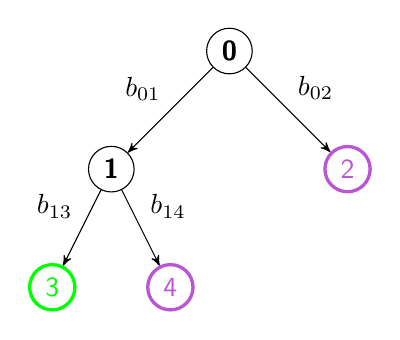
\begin{tikzpicture}[->,>=stealth',level/.style={sibling distance = 3cm/#1,
  level distance = 1.5cm}] 
\node [blackNode] {0} 
    child{ node [blackNode] {1}
            child{ node [greenNode] {3} edge from parent node[above left]{$b_{13}$} 
            }
            child{ node [purpleNode] {4} edge from parent node[above right]{$b_{14}$}				
            }
	    edge from parent node[above left]{$b_{01}$}
    }
    child{ node [purpleNode] {2} 
	edge from parent node[above right]{$b_{02}$}
    }
; 
\end{tikzpicture}
\caption{Example of a Branch-and-Price tree: Black nodes have been processed, the green node is the current active node, and purple are nodes which are waiting to be processed.}
\label{fig:bap_tree}
\end{figure}

By default, the $AbstractMaster$ and $AbstractPricingProblemSolver$ classes already implement this interface, and as a result, they are informed when a Branching Decision has been executed/reverted.\\
Returning to our TSP example, where we have two Branching Decisions, \code{RemoveEdge} and \code{FixEdge}, we are now ready to define what happens when either of them gets executed/reverted. When we execute a \code{RemoveEdge} Branching Decision, then the Pricing Problem defined in this Branching Decision can no longer produce matchings with this edge. Similarly, if we execute a \code{FixEdge} Branching Decision, then the Pricing Problem defined in this Branching Decision can only produce matchings which contain this edge. To implement this behavior, we need to modify our \code{ExactPricingProblemSolver} class (see \ref{codeBlock:tspExactPricingProblemSolver}), thereby adding the following two methods:

\begin{myblock}{ExactPricingProblemSolver continued}
\begin{lstlisting}[language=java, style=eclipseArticle, xleftmargin=2em]  
@Override
public void branchingDecisionPerformed(BranchingDecision bd) {
	if(bd instanceof FixEdge){
		FixEdge fixEdgeDecision = (FixEdge) bd;
		if(fixEdgeDecision.pricingProblem == this.pricingProblem)
			matchingSolver.fixEdge(fixEdgeDecision.edge); //Columns returned must contains this edge.
	}else if(bd instanceof RemoveEdge){
		RemoveEdge removeEdgeDecision= (RemoveEdge) bd;
		if(removeEdgeDecision.pricingProblem == this.pricingProblem)
			matchingSolver.removeEdge(removeEdgeDecision.edge); //Columns returned CANNOT contain this edge.
	}
}

@Override
public void branchingDecisionReverted(BranchingDecision bd) {
	if(bd instanceof FixEdge){
		FixEdge fixEdgeDecision = (FixEdge) bd;
		if(fixEdgeDecision.pricingProblem == this.pricingProblem)
			matchingSolver.undoFixEdge(fixEdgeDecision.edge);
	}else if(bd instanceof RemoveEdge){
		RemoveEdge removeEdgeDecision= (RemoveEdge) bd;
		if(removeEdgeDecision.pricingProblem == this.pricingProblem)
			matchingSolver.undoRemoveEdge(removeEdgeDecision.edge);
	}
}
\end{lstlisting}
\end{myblock}
Also in the \code{Master} class, a minor modification has to be made. The Master Problem currently maintains a set of columns. Some of these columns may not longer be valid when we start processing a new node. Two straightforward solutions exist:
\begin{enumerate}
 \item if a Branching Decision is executed, we iterate over all columns currently active in the Master model. For each column we test whether it is compliant with the Branching Decision. If not, we remove the column from the Master Problem. Remember that this compliance test can be performed using the \code{columnIsCompatibleWithBranchingDecision} method in the \code{BranchingDecision} class.
 \item simply destroy the current Master Problem and rebuild it.
\end{enumerate}
For the sake of simplicity we opt to go for the second approach, thereby adding the following method to the \code{Master} class:
\begin{myblock}{Master continued}
\begin{lstlisting}[language=java, style=eclipseArticle, xleftmargin=2em]  
@Override
public void branchingDecisionPerformed(BranchingDecision bd) {
	this.close(); //Invoke the destructor
	masterData=this.buildModel(); //Create a new model without any initialColumns
	cutHandler.setMasterData(masterData); //Inform the cutHandler about the new master model
}

@Override
public void branchingDecisionReverted(BranchingDecision bd) { } //No action required
\end{lstlisting}
\end{myblock}

The last class to extend is the \code{AbstractBranchAndPrice} class. This requires you to implement the following two methods:
\begin{itemize}
 \item \code{generateArtificialSolution} Details on this method are provided in Section \ref{subsec:initSolution}.
 \item \code{isIntegralSolution} this method determines whether a particular solution is an integer solution. In our case, an integer solution consist of 2 columns: one red matching and one blue matching, so we can safely conclude that if the master returns only 2 columns with a non-zero $z_m$ value, that the solution must be an integer solution.
\end{itemize}
The following code block gives the \code{BranchAndPrice} implementation.
\begin{myblock}{BranchAndPrice}
\begin{lstlisting}[language=java, style=eclipseArticle, xleftmargin=2em]  
public final class BranchAndPrice extends AbstractBranchAndPrice<TSP,Matching, PricingProblemByColor> {
    public BranchAndPrice(TSP modelData,
                          Master master,
                          List<PricingProblemByColor> pricingProblems,
                          List<Class<? extends AbstractPricingProblemSolver<TSP, Matching, PricingProblemByColor>>> solvers,
                          List<? extends AbstractBranchCreator<TSP, Matching, PricingProblemByColor>> branchCreators,
                          int upperBoundOnObjective,
                          List<Matching> initialSolution){
        super(modelData, master, pricingProblems, solvers, branchCreators, upperBoundOnObjective, initialSolution);
    }

    @Override
    protected List<Matching> generateArtificialSolution() {<Code Omitted>}

    @Override
    protected boolean isIntegerNode(BAPNode<TSP,Matching> node) {return node.getSolution().size()==2;}
}
\end{lstlisting}
\end{myblock}


Finally, we can bring all the parts together in a solver class:
\begin{myblock}{TSPSolver}
\begin{lstlisting}[language=java, style=eclipseArticle, xleftmargin=2em]  
public final class TSPSolver {
	public TSPSolver(TSP tsp){
		//Create a cutHandler, then create a Subtour AbstractInequality Generator and add it to the handler
		CutHandler<TSP, TSPMasterData> cutHandler=new CutHandler<>();
		SubtourInequalityGenerator cutGen=new SubtourInequalityGenerator(tsp);
		cutHandler.addCutGenerator(cutGen);

		//Create the two Pricing Problems
		List<PricingProblemByColor> pricingProblems=new ArrayList<>();
		pricingProblems.add(new PricingProblemByColor(tsp, "redPricing", MatchingColor.RED));
		pricingProblems.add(new PricingProblemByColor(tsp, "bluePricing", MatchingColor.BLUE));

		//Create the Master Problem
		Master master=new Master(tsp, pricingProblems, cutHandler);
		
		//Define which solvers to use
		List<Class<? extends AbstractPricingProblemSolver<TSP, Matching, PricingProblemByColor>>> solvers= Collections.singletonList(ExactPricingProblemSolver.class);
		
		//OPTIONAL: Get an initial solution and use it as an upper bound
		List<Matching> initSolution=<Code Omitted>

		//Define one or more Branch creators
		List<? extends AbstractBranchCreator<TSP, Matching, PricingProblemByColor>> branchCreators= Collections.singletonList(new BranchOnEdge(tsp, pricingProblems));

		//Create a Branch-and-Price instance
		BranchAndPrice bap=new BranchAndPrice(tsp, master, pricingProblems, solvers, branchCreators, initObjective, initSolution);

		//OPTIONAL: Attach a debugger
		SimpleDebugger debugger=new SimpleDebugger(bap, cutHandler, true);

		//OPTIONAL: Attach a logger to the Branch-and-Price procedure.
		SimpleBAPLogger logger=new SimpleBAPLogger(bap, new File("./tsp.log"));

		//Solve the TSP problem through Branch-and-Price
		bap.runBranchAndPrice(System.currentTimeMillis()+8000000L);

		//Print solution:
		<Code Omitted>

		//Clean up:
		bap.close(); //Close master and Pricing Problems
		cutHandler.close(); //Close the cut handler. The close() call is propagated to all registered AbstractCutGenerator classes
	}
}
\end{lstlisting}
\end{myblock}


\section{Implementation details}

\subsection{Column Generation solve method}
Figure \ref{fig:cg_flowChart} gives a possible flow of the \code{solve} method in the \code{ColGen} class. First the Master Problem is solved. Then a check is performed whether the solve procedure may be terminated based on any of the bounds (see Section \ref{subsec:bounds}). After that the Pricing Problem is solved. Two algorithms are provided for this purpose: if the first algorithm fails to identify columns with negative reduced cost, the second algorithm gets invoked. After one or more columns are returned, a bound on the optimal solution of the Master Problem may be calculate. When no columns are returned, the Master Problem is per definition solved to optimality. The \code{CutHandler} is invoked to check whether the current solution of the Master Problem violates any valid inequalities. If this is the case, these inequalities are added to the Master Problem and a new Column Generation iteration is started. If no inequalities are violated, the Column Generation procedure terminates.

\begin{figure}[h!]
  \caption{Flow chart of Column Generation procedure.}
  \centering
    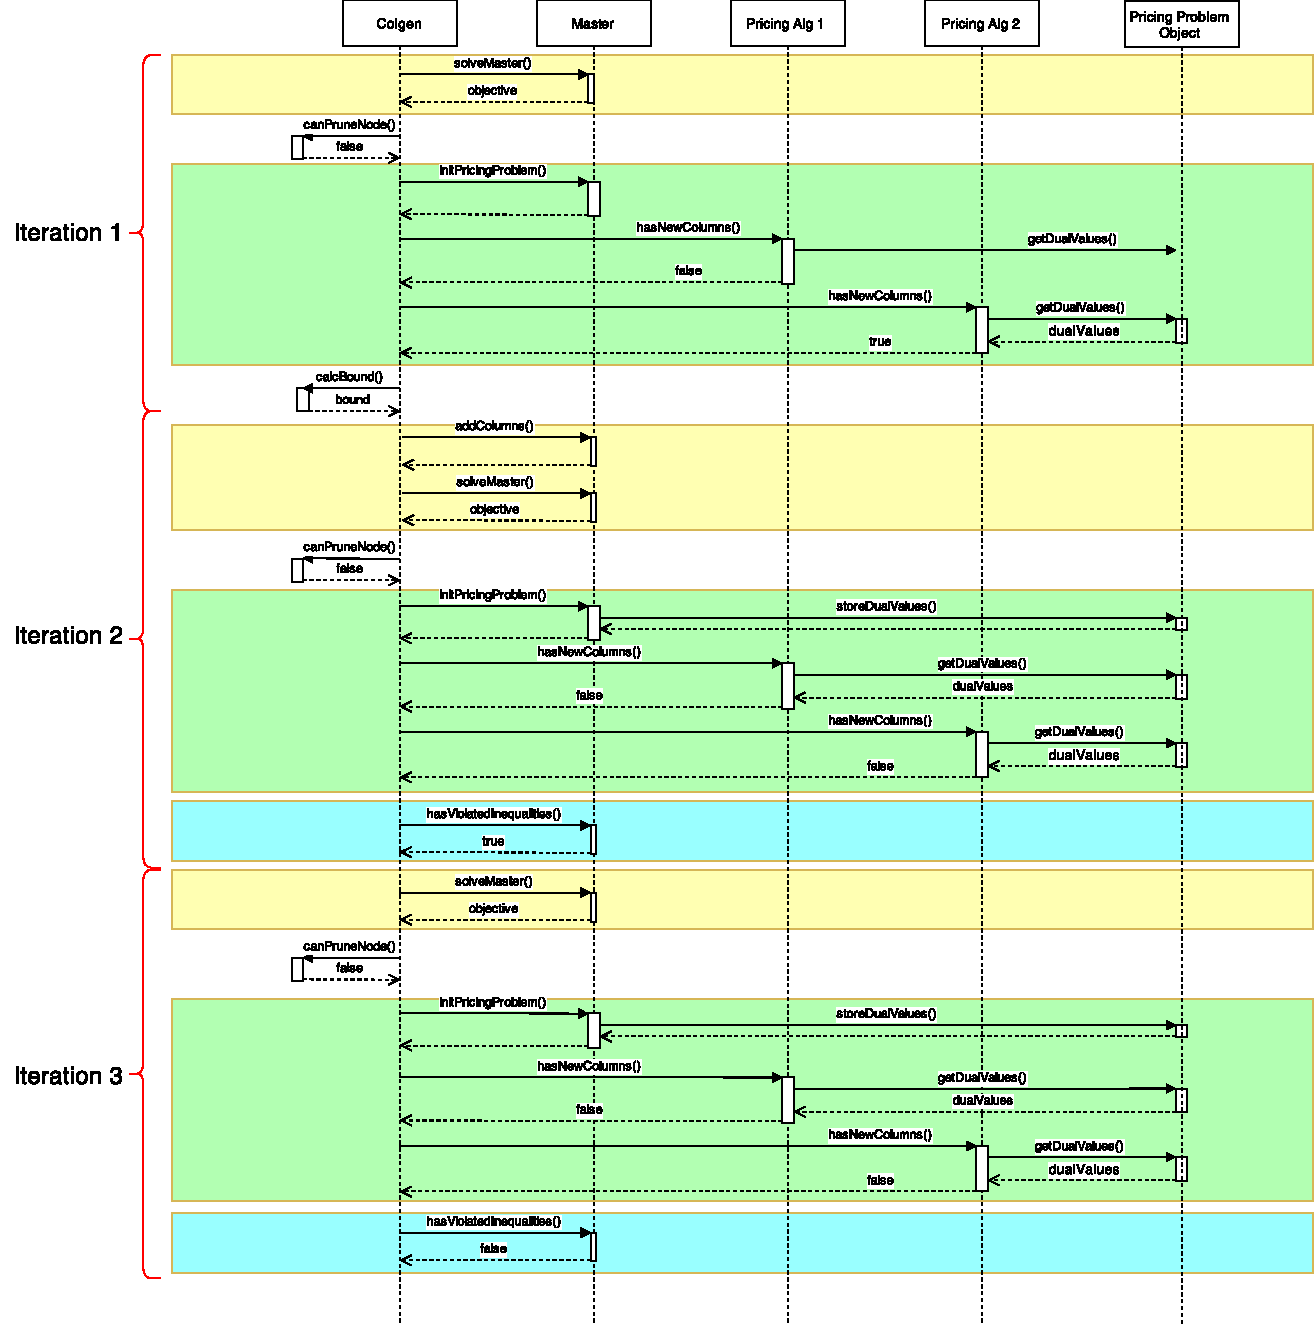
\includegraphics[width=0.8\textwidth]{figures/CG_flowChart}
  \label{fig:cg_flowChart}
\end{figure}

\subsection{Branch-and-Price solve method}
The \code{AbstractBranchAndPrice} class implements a solve method which processes Branch-and-Price nodes from a queue until the queue is empty, or a time limit is reached. After solving a node, the following 4 conditions may hold:
\begin{itemize}
 \item the node is infeasible (no solution to its Master Problem exists)
 \item the node is integer. The best integer solution is recorded.
 \item the node is fractional. The bound on the node is compared with the best integer solution; if the bound exceeds the best integer solution, the node is pruned. Otherwise, branching is performed, thereby creating two or more child nodes which are added to the queue.
 \item the status of the node is unknown: this may for example occur when the node is being solved while the time limit is reached. The node is placed back into the queue. 
\end{itemize}



\subsection{Bounds}\label{subsec:bounds}
To speed up the CG procedure, bounds can be computed on the optimal solution. These bounds are often problem dependent; hence no standard implementation is provided. However, the framework supports the calculation of bounds in various ways. A valid bound on the optimal CG objective is frequently calculated by combining information from the Master Problem, and information from the the Pricing Problems (the optimal solution to the Pricing Problem, or a bound thereof).
\begin{itemize}
 \item Information from the Master Problem can be queried through the function: \code{getBoundComponent}.
 \item Each \code{AbstractPricingProblemSolver} has a method \code{getBound}. If a particular\\ \code{AbstractPricingProblemSolver} solves the Pricing Problem to optimality, the \code{getBound} function would typically return the optimal solution. Alternatively, the objective value of a relaxation of the Pricing Problem may be returned, e.g. the LP relaxation when the Pricing Problem is implemented as a MIP, or the value of a Lagrangian Relaxation.
 \item When there are multiple Pricing Problems, multiple bounds on these Pricing Problems may be queried in parallel through the \code{getBoundsOnPricingProblems} method in the \code{PricingProblemManager}. The latter is accessible through the \code{ColGen} class (or an extension thereof). The number of parallel threads used to calculate these bounds are specified in the \code{Configuration} class.
 \item To calculate a bound on the optimal value of the Master Problem, the method\\ \code{calculateBoundOnMasterObjective} is provided in the \code{ColGen} class. This method has access to the aforementioned methods.
\end{itemize}
The default implementation of the class \code{ColGen} provided in the framework terminates the \code{solve} procedure under the following conditions:
\begin{enumerate}
 \item No more columns are returned by the Pricing Problem(s) (and no inequalities are violated): Solved to optimality
 \item Time limit exceeded (throws exception)
 \item If the optimality gap is closed, i.e. the objective of the Master Problem equals the bound calculated on the optimal solution of the Master Problem (see \code{getBound} method in ColGen class).
 \item If the bound on the Master Problem objective exceeds the cutoff value which was provided during the construction of the \code{ColGen} instance. In the context of Branch-and-Price, one often has a incumbent solution to the original problem. A node in the Branch-and-Price tree may be pruned if its bound exceeds the value of the incumbent solution. Therefore, an integer solution (cutoff value) may be provided to the Column Generation procedure.
\end{enumerate}
Obviously, any of the above conditions may be modified by overriding the \code{solve} method with a custom implementation.\\
Note: bounds computed at various iterations of the column generation procedure are usually not monotonically increasing in strength. That is, the bound calculated at iteration $i$ may be stronger than the bound calculated at iteration $j$, $j>i$. The framework keeps track of the strongest bound.


\subsection{Solving the Pricing Problem(s)}\label{sec:colGen}
The \emph{Pricing Problem} defines under which conditions a new column has to be added to the \emph{Master Problem}. Each Pricing Problem has to be solved by some algorithm which is defined as a \code{PricingProblemSolver}. Multiple algorithms may be specified in a hierarchical fashion. One can for example specify a fast heuristic Pricing Problem solver. If the heuristic solver fails, one can fall back on an exact solver.\\
Very often, a column generation procedure consist of one Master Problem, and multiple independent Pricing Problems. The Pricing Problems are automatically solved in parallel; no interference of the user is required (the number of threads for parallel execution can be specified through the \code{Configuration} class). An example of a problem with multiple, independent Pricing Problems is given in Section \ref{sec:tsp}.


 
\subsection{Initial solution}\label{subsec:initSolution}
Any node in the Branch-and-Price tree must be initialized with an initial feasible solution, i.e.\ a subset of columns which provide an initial feasible solution to the restricted Master Problem. Alternatively, when such a set of columns does not exist, one needs to prove infeasibility of the Master Problem. The root node can be straightforwardly initialized by any feasible solution to the optimization problem, but finding an initial feasible solution for any of its siblings tends to be difficult. Moreover, proving that such a solution does not exist is a cumbersome task. In fact, finding such a solution is about as hard as solving the actual optimization problem you are trying to solve in the first place. Hence it would be beneficial when the Master Problem itself could be used to prove nonexistence of a feasible solution. With this goal in mind, \emph{artificial columns},
which together meet all the constraints of the Master Problem, are introduced. Each artificial column has a cost strictly larger than the cost of any non-artificial column; hence, the Master Problem favors cheaper
non-artificial columns over the artificial ones. When the column generation procedure terminates, and the resulting solution still contains artificial columns, one can conclude that no feasible solution exists as they would have been generated by the Pricing Problem.\\
Artificial columns can be added to the Branch-and-Price implementation by setting the \emph{isArtificial} field to true (see the \code{AbstractColumn} class for details). If a solution to any of the nodes in the Branch-and-Price tree contains an artificial column, the node is automatically pruned and marked as "infeasible".

\subsection{Branch-and-Price node ordering}
The nodes in a Branch-and-Price tree may be processed in an arbitrary order. The default implementation uses a Depth-First-Search processing order. Nevertheless, a user may provide a custom ordering. To do so, a \code{Comparator<BAPNode>} must be implemented. Two examples are provided in the classes \code{BFSbapNodeComparator} and \code{DFSbapNodeComparator} respectively. The comparator must be provided to the Branch-and-Price implementation through the \code{setNodeOrdering} method in the class \code{AbstractBranchAndPrice}.\\


\section{Miscellaneous topics}

\subsection{Logging and Debugging}
Each class in the framework is equipped with a logger. For details refer to the documentation of Logback (\cite{logback}) and SLF4j (\cite{slf4j}). In addition, the classes \code{ColGen}, \code{AbstractBranchAndPrice} and \code{CutHandler} are equipped with a notifier which fires events during various stages of the Branch-and-Price and Column Generation procedures. These events can be captured by resp.\ a \code{CGListener}, \code{BAPListener} and \code{CHListener}. Examples of a logger and a debugger are provided by the \code{SimpleBAPLogger}, \code{SimpleCGLogger} and \code{SimpleDebugger} classes.

\subsection{Configuration}
A number of parameters may be configured through the \code{Configuration} class, including the number of threads used to solve the Pricing Problems, and whether valid inequalities should be separated or not. The configuration files can be accessed through the \code{AbstractMaster}, \code{AbstractPricingProblemSolver}, \code{CutHandler} classes. The user may also specify custom configurations, as well as additional parameters. 



\bibliographystyle{IEEEtranS} %IEEEtranS
%\bibliographystyle{IEEEtranSN} %IEEEtranS %model2-names
\bibliography{sources}


\end{document}
